\documentclass[border=0pt]{standalone}
\usepackage{amsmath}
\usepackage[usenames,dvipsnames]{xcolor}
\usepackage{graphicx}

%%font
\usepackage{euler}
\usepackage[OT1]{eulervm}
\renewcommand{\rmdefault}{pplx}

\usepackage{amsmath, amssymb}
\usepackage{bigints}
\usepackage[hidelinks]{hyperref}

\newcommand{\bx}{\mathbf{x}}
\newcommand{\by}{\mathbf{y}}
\newcommand{\bu}{\mathbf{u}}
\newcommand{\bv}{\mathbf{v}}

\setcounter{MaxMatrixCols}{20}

\usepackage{tikz}
\tikzset{roundnode/.style={circle,draw=black,fill=blue!20}, 
every label/.style={rectangle, draw=none}}
\definecolor{TortugaColor}{rgb}{0.1,0.4,0.3}
\definecolor{Totemblue}{HTML}{09182F}
\definecolor{Totemred}{HTML}{2B030B}
\definecolor{Totemyellow}{HTML}{AD901B}
\definecolor{ILASgold}{HTML}{e9d387}
\usetikzlibrary{intersections}
%\usetikzlibrary{fadings}
\usetikzlibrary{arrows}
%\usetikzlibrary{arrows.meta}
%\usetikzlibrary{decorations}
\usetikzlibrary{decorations.pathmorphing}
\usetikzlibrary{decorations.text}
%% \usetikzlibrary{shadings}
%\usetikzlibrary{fit}
%\usetikzlibrary{calc}
%\usetikzlibrary{through}
%\usetikzlibrary{positioning}
%\usetikzlibrary{graphs}
%\usetikzlibrary{mindmap}
%\usetikzlibrary{backgrounds}
%\usetikzlibrary{calligraphy}
%% \usepgfmodule{nonlineartransformations}
%% \usetikzlibrary{curvilinear}

%%% Set up polar step (code from the pgd manual)
%\makeatletter
%\def\polartransformation{%
% \pgf@x will contain the radius
% \pgf@y will contain the distance
%\pgfmathsincos@{\pgf@sys@tonumber\pgf@x}%
% pgfmathresultx is now the cosine of radius and
% pgfmathresulty is the sine of radius
%\pgf@x=\pgfmathresultx\pgf@y%
%\pgf@y=\pgfmathresulty\pgf@y%
%}
%\makeatother

\pgfdeclarelayer{background}
\pgfdeclarelayer{alpha}
\pgfdeclarelayer{beta}
\pgfsetlayers{background,alpha,main,beta}

%%pic TaiJi
\tikzset{
TaiJi/.pic={
\begin{scope}[thick,yi/.style={radius=0.4cm}]
\shade [draw=black] (0,0) circle [radius =3];
\shade [top color=black, bottom color=black!50,draw=black] (0,-3) arc [radius=3, start angle=-90, end angle=90]
arc [radius=1.5, start angle=90, end angle=270]
arc [radius=1.5, start angle=90, end angle=-90];
\draw[thin,fill=black] (0,-1.5) circle [yi];
\draw[thin,fill=white] (0,1.5) circle [yi];
\end{scope}
}}

%%pic Totu
\tikzset{
totu/.pic={
\begin{scope}[scale=0.2]
\pgfmathsetmacro{\legwidth}{0.4*0.2}
\draw[fill=green!60!black!30] (0,0.8) circle [x radius=0.3,y radius=0.4];
\foreach \i in {-1,1}{
\begin{scope}[xscale=\i]
\path (0.8,0) edge[draw=green!60!black!30,line width=\legwidth cm,line cap=round,bend left] ++(0.6,0);
\path (0.6,-1) edge[draw=green!60!black!30,line width=\legwidth cm,line cap=round] ++ (0.4,-0.4);
\end{scope}
}
\draw (0,-1.4) edge[draw=green!60!black!30,line width=\legwidth cm,line cap=round] ++ (0,-0.4);
\draw[fill=green!60!black,rounded corners] (1,0) -- (0,0.5) -- (-1,0) -- (-0.8,-1.2) -- (0,-1.6) -- (0.8,-1.2) -- cycle;
\end{scope}
}}

%%pic Rescuer
\tikzset{
Rescuer/.pic={
\begin{scope}[shift={(6.35,1.2)}]
\draw[fill=black!20!red!60!yellow] (-7,-0.8) -- (-6.7,-1.2) -- (-6,-1.2) -- (-5.7,-0.8) .. controls +(-0.3,-0.1) and +(0.3,-0.1) ..  cycle;
\end{scope}
}}

%%pic SatanHeart
\tikzset{
SatanHeart/.pic={
\pgfmathsetmacro{\SatanHradius}{1}
\pgfmathsetmacro{\LSatanHradius}{1.05}
\begin{scope}[very thick]
\draw[gray!80!blue, line width=2pt] (0,0) circle[radius=\LSatanHradius cm];
\draw[gray!80!blue] (-90:\SatanHradius) -- (-306:\SatanHradius) -- (-162:\SatanHradius) -- (-378:\SatanHradius) -- (-234:\SatanHradius) -- cycle;
\end{scope}
}}

%%pic Stone Gate
\tikzset{
stonegate/.pic={
\begin{scope}[gray]
\draw[fill,draw=none,rounded corners] (-1.3,-0.3) rectangle (-0.7,2);
\draw[fill,draw=none,rounded corners] (0.7,-0.3) rectangle (1.3,2);
\draw[fill,draw=none] (0,2) ellipse[x radius=2cm, y radius=0.3cm];
\end{scope}
}}
 
%%pic Ateles Zombia
\tikzset{
zombia/.pic={
\pgfmathsetmacro{\zombiascale}{0.2}
\begin{scope}[scale=\zombiascale]
\pgfmathsetmacro{\zombiawidth}{\zombiascale *0.3 cm}
\pgfmathsetmacro{\zombiabigcorner}{\zombiascale *4 pt}
\pgfmathsetmacro{\zombiasmallcorner}{\zombiascale *0.2 cm}
\begin{scope}[gray!40, rounded corners=\zombiabigcorner, line width=\zombiawidth, line cap=round]
%\node[circle,draw,thin] at (0,0) {};
\draw [fill,thin] (-1.9,0.4) circle [radius=0.3cm];
\draw (-1.8,0.1) -- (-2.2,-0.3) -- (-2.7,-0.6);
\draw (-1.8,0.1) -- (-1.6,-0.8) -- ++ (0.1,-0.1);
\draw (-1.8,0.1) -- (-0.9,0.1) -- (0.4,0.8);
\draw[rounded corners=\zombiasmallcorner] (0.4,0.8) -- ++ (0.3,0.2) -- ++ (0.2,-0.2);
\draw (0.7,1) -- (0.9,1.3) -- (1,2.5) -- (1.3,3) -- (1.8,2.9);
\draw (0.9,0.8) -- (0.9,0.5) -- (0.95,-0.3) -- (0.8,-1.1);
\draw (0.8,0.8) -- (0.4,0.6) -- (0,-0.7) -- ++(-0.2,-0.2);
\end{scope}
\end{scope}
}
}

%%pic family
\tikzset{
family/.pic={
\begin{scope}[xshift=-1cm]
\clip (0,0) rectangle (2,1);
\draw[fill] (0.25,0.7) circle [radius=0.1cm];
\draw[line cap=round,line width=0.06cm] (0.25,0.7) -- (0.25,0.2);
\draw[line cap=round,line width=0.06cm] (0.15,0) -- (0.25,0.2) -- (0.35,0);

\draw[fill] (0.75,0.6) circle [radius=0.1cm];
\draw[line cap=round,line width=0.06cm] (0.75,0.6) -- (0.75,0.2);
\draw[line cap=round,line width=0.06cm] (0.65,0) -- (0.75,0.2) -- (0.85,0);

\draw[fill] (1.25,0.6) circle [radius=0.1cm];
\draw[line cap=round,line width=0.06cm] (1.25,0.6) -- (1.25,0.2);
\draw[line cap=round,line width=0.06cm] (1.15,0) -- (1.25,0.2) -- (1.35,0);

\draw[fill] (1.75,0.65) circle [radius=0.1cm];
\draw[line cap=round,line width=0.06cm] (1.75,0.65) -- (1.75,0.2);
\draw[line cap=round,line width=0.06cm] (1.65,0) -- (1.75,0.2) -- (1.85,0);

\draw[line cap=round, line width=0.06cm] (0,0.3) -- (0.25,0.5) -- (0.5,0.3) -- (0.75,0.4) -- (1,0.3) -- (1.25,0.4) -- (1.5,0.3) -- (1.75,0.45) -- (2,0.3);
\end{scope}
}
}

\parindent=0pt

\begin{document}
%%2025NewYear
%% 16:9
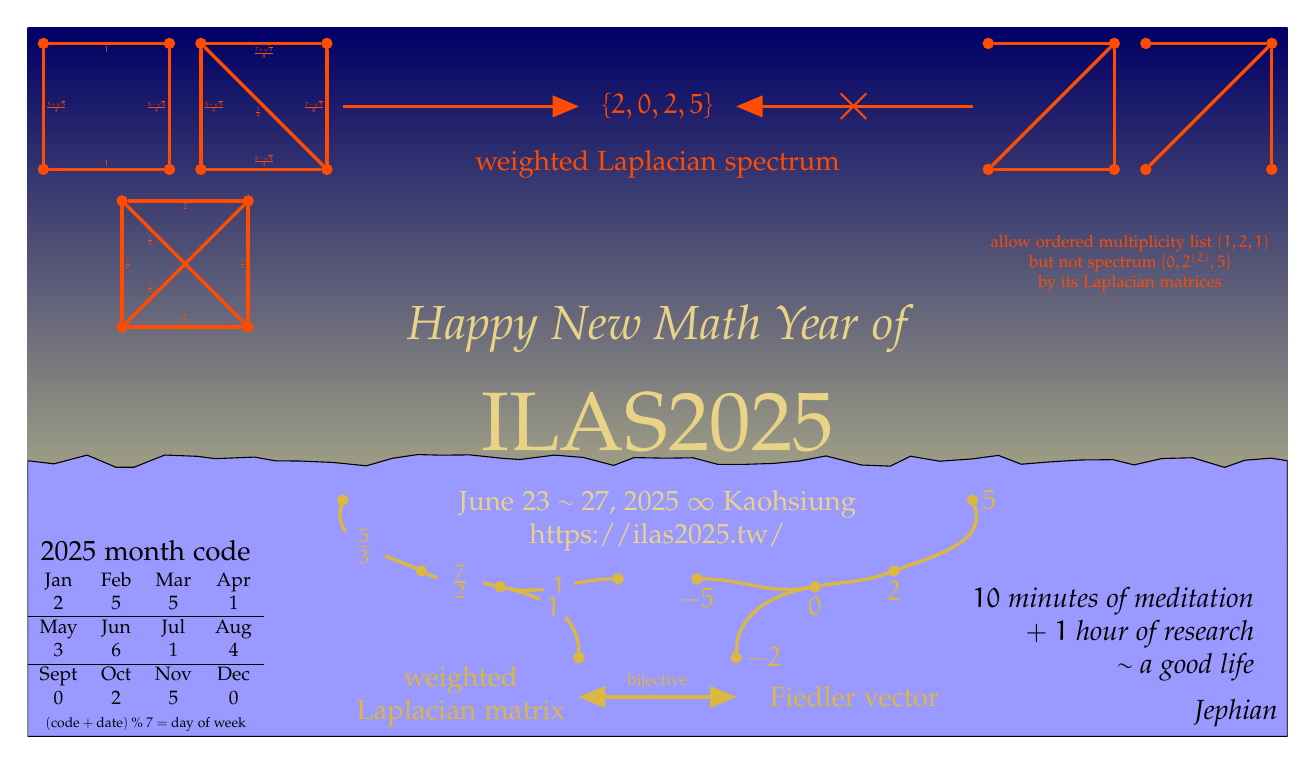
\begin{tikzpicture}
\coordinate (Jamaica) at (-8,-4);
\coordinate (Dominican) at (8,-4);
\coordinate (Cuba) at (-8,5);
\coordinate (TurksCaicos) at (8,5);
\coordinate (Tortuga) at (0,0);
\clip (Jamaica) rectangle (TurksCaicos);

%%Help Lines
\begin{pgfonlayer}{beta}
%% \draw [step=1, black!50, thin] (Jamaica) grid (TurksCaicos);
%% \draw (0,0) circle [radius=0.2cm];
\end{pgfonlayer}


%%background Layer
\begin{pgfonlayer}{background}
\shade [top color=blue!40!black, bottom color=yellow!40] (-8,-4) rectangle (8,5);
%% \shade [inner color=yellow!40, outer color=blue!40!black] (-8,-4) rectangle (8,5);
%% \shade [left color=orange, right color=red!70] (-8,-4) rectangle (8,5);
%% \shade [shading=axis, top color=orange!50, bottom color=red!50, shading angle=135] (-8,-4) rectangle (8,5);
%% \begin{scope}[opacity=0.2]
%% \foreach \i in {1,2,3,4} {
%%     \pgfmathsetmacro{\ang}{180 - 18 * \i}
%%     \pgfmathsetmacro{\rang}{180 + \ang}
%%     \pic[xshift=-0.5cm, rotate=\rang] at (\ang:3) {totu};
%% }
%% \foreach \i in {1,2,3,4} {
%%     \pgfmathsetmacro{\ang}{270 + 18 * \i}
%%     \pgfmathsetmacro{\rang}{\ang}
%%     \pic[xshift=0.5cm, rotate=\rang] at (\ang:3) {totu};
%% }
%% \end{scope
%% }
\end{pgfonlayer} 


%%Main Layer (main)
\begin{pgfonlayer}{main}

%%Sea
\draw[fill=blue!40,name path=sealevel] decorate[decoration={name=random steps}] {(0,-0.5 -| Jamaica) -- (0,-0.5 -| Dominican)} -- (Dominican) -- (Jamaica) -- cycle;


\begin{scope}
[red!40!orange, 
every node/.style={circle, draw, fill, inner sep=1pt}, very thick, 
weight/.style={rectangle, draw=none, fill=none, scale=0.3, inner sep=3pt}]

%% C4
\begin{scope}[shift={(-7,4)}]
\node (c41) at (-0.8,0.8) {};
\node (c42) at (0.8,0.8) {};
\node (c43) at (0.8,-0.8) {};
\node (c44) at (-0.8,-0.8) {};
\draw (c41) --node[midway,weight,below]{$1$} (c42);
\draw (c42) --node[midway,weight,left]{$\frac{5-\sqrt{5}}{4}$} (c43);
\draw (c43) --node[midway,weight,above]{$1$} (c44);
\draw (c44) --node[midway,weight,right]{$\frac{5+\sqrt{5}}{4}$} (c41);
\end{scope}

%% K4-e
\begin{scope}[shift={(-5,4)}]
\node (k4e1) at (-0.8,0.8) {};
\node (k4e2) at (0.8,0.8) {};
\node (k4e3) at (0.8,-0.8) {};
\node (k4e4) at (-0.8,-0.8) {};
\draw (k4e1) --node[midway,weight,below]{$\frac{7+\sqrt{5}}{8}$} (k4e2);
\draw (k4e2) --node[midway,weight,left]{$\frac{7-\sqrt{5}}{8}$} (k4e3);
\draw (k4e3) --node[midway,weight,above]{$\frac{5-\sqrt{5}}{4}$} (k4e4);
\draw (k4e4) --node[midway,weight,right]{$\frac{5+\sqrt{5}}{4}$} (k4e1);
\draw (k4e1) --node[midway,weight,anchor=45]{$\frac{1}{4}$} (k4e3);
\end{scope}

%% K4
\begin{scope}[shift={(-6,2)}]
\node (k41) at (-0.8,0.8) {};
\node (k42) at (0.8,0.8) {};
\node (k43) at (0.8,-0.8) {};
\node (k44) at (-0.8,-0.8) {};
\draw (k41) --node[midway,weight,below]{$2$} (k42);
\draw (k42) --node[midway,weight,left]{$\frac{1}{2}$} (k43);
\draw (k43) --node[midway,weight,above]{$\frac{1}{2}$} (k44);
\draw (k44) --node[midway,weight,right]{$\frac{1}{2}$} (k41);
\draw (k41) --node[near start,weight,anchor=45]{$\frac{1}{2}$} (k43);
\draw (k42) --node[near end,weight,anchor=-45]{$\frac{1}{2}$} (k44);
\end{scope}

%% K13
\begin{scope}[shift={(7,4)}]
\node (k131) at (-0.8,0.8) {};
\node (k132) at (0.8,0.8) {};
\node (k133) at (0.8,-0.8) {};
\node (k134) at (-0.8,-0.8) {};
\draw (k132) -- (k131);
\draw (k132) -- (k133);
\draw (k132) -- (k134);
\end{scope}

%% Paw
\begin{scope}[shift={(5,4)}]
\node (paw1) at (-0.8,0.8) {};
\node (paw2) at (0.8,0.8) {};
\node (paw3) at (0.8,-0.8) {};
\node (paw4) at (-0.8,-0.8) {};
\draw (paw2) -- (paw1);
\draw (paw2) -- (paw3);
\draw (paw2) -- (paw4);
\draw (paw3) -- (paw4);
\end{scope}



\node[rectangle, draw=none, fill=none] (spec) at (0,4) {$\{2,0,2,5\}$};
\node[rectangle, draw=none, fill=none, below=0.5cm] (spec.south) at (0,4) {weighted Laplacian spectrum};
\draw[very thick, -triangle 45] (-4,4) -- (-1,4);
\draw[very thick, -triangle 45] (4,4) --node[midway,draw=none,fill=none,scale=2] {$\times$} (1,4);
\end{scope}

% text: allow (1,2,1)
\node[draw=none, red!40!orange, align=center, scale=0.6] at (6,2) {allow ordered multiplicity list $(1,2,1)$\\but not spectrum $\{0,2^{(2)},5\}$\\by its Laplacian matrices};

%% \node[draw=none] at (6,2) {
%%   \href{https://ilas2025.tw/}{
%%     \tikz\node[red!40!orange, draw=none, rectangle, align=center, scale=0.6] at (0,0) {allow ordered multiplicity list $(1,2,1)$\\but not spectrum $\{0,2^{(2)},5\}$\\by its Laplacian matrices};
%%   }
%% };

\begin{scope}
[xscale=1, 
yellow!40!brown, 
every node/.style={circle, draw, fill, inner sep=1pt}, 
very thick,
every label/.style={draw=none, fill=none, rectangle}]
\node[label={below:$-5$}] (rs0) at (0.5,-2) {};
\node[label={right:$-2$}] (rs1) at (1,-3) {};
\node[label={below:$0$}] (rs2) at (2,-2.1) {};
\node[label={below:$2$}] (rs3) at (3,-1.9) {};
\node[label={right:$5$}] (rs4) at (4,-1) {};
\draw[out=0, in=190] (rs0) to (rs2);
\draw[out=90, in=190] (rs1) to (rs2);
\draw[out=10, in=200] (rs2) to (rs3);
\draw[out=20, in=290] (rs3) to (rs4);
\end{scope}

\begin{scope}
[xscale=-1, 
yellow!40!brown, 
every node/.style={circle, draw, fill, inner sep=1pt}, 
very thick,
every label/.style={draw=none, fill=none, rectangle}]
\node (rs0) at (0.5,-2) {};
\node (rs1) at (1,-3) {};
\node (rs2) at (2,-2.1) {};
\node (rs3) at (3,-1.9) {};
\node (rs4) at (4,-1) {};
\draw[out=0, in=190] (rs0) to node[midway,draw=none,fill=blue!40] {$1$} (rs2);
\draw[out=90, in=190] (rs1) to node[midway,draw=none,fill=blue!40] {$1$} (rs2);
\draw[out=10, in=200] (rs2) to node[midway,draw=none,fill=blue!40] {$\frac{7}{2}$} (rs3);
\draw[out=20, in=290] (rs3) to node[midway,draw=none,fill=blue!40] {$\frac{5}{3}$} (rs4);
\end{scope}

\begin{scope}[yellow!40!brown, very thick]
\node[align=center] at (-2.5,-3.5) {weighted\\Laplacian matrix};
\node at (2.5,-3.5) {Fiedler vector};
\draw[triangle 45-triangle 45] (-1,-3.5) --node[midway, above, rectangle, scale=0.6] {bijective} (1,-3.5);
\end{scope}
%% cwp

\end{pgfonlayer}


%%beta layer
\begin{pgfonlayer}{beta}
%% ILAS2025
\node[rectangle, draw=none, ILASgold, scale=3] (ILAS2025) at (0,0) {ILAS2025};
\node[rectangle, draw=none, ILASgold, below, scale=1, align=center] (ILAStime) at (ILAS2025.south) {June 23 $\sim$ 27, 2025 $\infty$ Kaohsiung\\\url{https://ilas2025.tw/}};


%%Happy New Math Year
%\draw[decorate,decoration={text along path,text={|\color{red!80!yellow} \LARGE \it|Happy New Math Year 2020}}] (-3.5,-2.5) .. controls (-1,4.5) and (1,4.5) .. (3.5,-2.5);
%% \node[rectangle, draw=none, orange!80!yellow] at (0,-3) {\LARGE\it Happy New Math Year 2023};
\node[rectangle, draw=none, ILASgold, above] (hny) at (ILAS2025.north) {\LARGE\it Happy New Math Year of};
%% \draw[yellow, very thick, -triangle 45, shorten <=0.1cm, shorten >=0.1cm] (hny.20) .. controls ++(0,2) and ++(0,-2) .. (2023.south);
%% \node[rectangle, draw=none, opacity=0] at (0,-0.5) {\Huge\tt FREE HONG KONG};

%%Month code
\node[above] at (-6.5,-1.9) {2025 month code};
\node[scale=0.7,below] at (-6.5,-1.8) {\begin{tabular}{cccc} 
Jan & Feb & Mar & Apr \\
 2 & 5 & 5 & 1 \\
\hline
May & Jun & Jul & Aug \\
 3 & 6 & 1 & 4 \\
\hline
Sept & Oct & Nov & Dec \\
 0 & 2 & 5 & 0 \\
\end{tabular}};
\node[scale=0.5,above] at (-6.5,-4) {$(\text{code}+\text{date})\mathbin{\%}7=\text{day of week}$};

%%Goal
% y 1.3 for three sentences
\node[yshift=1.3cm, xshift=-0.3cm, left, align=right] at (Dominican) {
\it $10$ minutes of meditation \\
\it $+$ $1$ hour of research \\
\it $\sim$ a good life};

%%Signature
\node[yshift=0.3cm,left] at (Dominican) {\it Jephian};

\end{pgfonlayer}




\end{tikzpicture}
\end{document}


%%\draw=\path[draw]
%%\clip=\path[clip]
%%\graph=\path[graph]
%%bend right ~ bend right=30 ~ in,out=right30, left 30
%%(left:2)=(180:2)
%%left ~ anchor=east ~ anchor 0
%%for sharp corners: line cap, line joint
%%for elliptical rectangle: smooth circle, plot coordinates, tensions
%For updating 2.10 to 3.0.0
%after moving the folder, it requires 
%sudo texhash 
% to make it work.
%%To convert to jpg: compile the pdf first, and then use the command below
%% convert -density 300 file.pdf -quality 90 file.jpg
%% required to install imagemagick

%% use pdf2png in AUR with Resolution 500 for 2018 
%% use gimp for 2019 (resolution 1890 x 1062, export quality 90)

%% Sample transformation as below
\makeatletter
\def\mytrans{
    \pgfmathparse{\pgf@x+1cm}
    %\pgf@x=\pgfmathresult pt
    \pgfmathsetlength{\pgf@x}{\pgfmathresult pt}
}
\makeatother
